%==============================================================================
\chapter{Quality Assessment of RDF Datasets at Scale}
\label{chapter:dist_quality_assessment}
%==============================================================================
Large amounts of data are being published openly to Linked Data by different data providers. 
A multitude of applications such as semantic search, query answering, and machine reading~\cite{rw2014} depend on these large-scale\furl{http://lodstats.aksw.org/} \gls{RDF} datasets.  
The quality of underlying \gls{RDF} data plays a fundamental role in large-scale data consuming applications. 
Measuring the quality of linked data spans a number of dimensions including but not limited to: accessibility, interlinking, performance, syntactic validity or completeness~\cite{zaveri2015quality}.
Each of these dimensions can be expressed through one or more quality metrics. 
Considering that each quality metric tries to capture a particular aspect of the underlying data, numerous metrics are usually provided against the given data that may or may not be processed simultaneously.

On the other hand, the limited number of existing techniques of quality assessment for \gls{RDF} datasets are not adequate to assess data quality at large-scale and these approaches mostly fail to capture the increasing volume of big data. 
To date, a limited number of solutions have been conceived to offer a quality assessment of \gls{RDF} datasets \cite{Debattista0AC18,farber2018,beek2018,debattista2016luzzu}.
But, these methods can either be used on a small portion of large datasets \cite{farber2018} or narrow down to specific problems e.g., syntactic accuracy of literal values~\cite{beek2018}, or accessibility of resources~\cite{Mihindukulasooriya2016LDSA}.
In general, these existing efforts show severe deficiencies in terms of performance when data grows beyond the capabilities of a single machine.
This limits the applicability of existing solutions to medium-sized datasets only, in turn, paralyzing the role of applications in embracing the increasing volumes of the available datasets.

To deal with big data, tools like Apache Spark\furl{https://spark.apache.org/} have recently gained a lot of interest. 
Apache Spark provides scalability, resilience, and efficiency for dealing with large-scale data. 
Spark uses the concepts of \gls{RDD}~\cite{zaharia2012resilient} and performs operations like transformations and actions on this data in order to effectively deal with large-scale data. 

To handle large-scale \gls{RDF} data, it is important to develop flexible and extensible methods that can assess the quality of data at scale. 
At the same time, due to the broadness and variety of quality assessment domain and resulting metrics, there is a strong need to provide a generic pattern to characterize the quality assessment of \gls{RDF} data in terms of scalability and applicability to big data.

In this chapter, we borrow the concepts of data \textit{transformation} and \textit{action} from Spark and present a pattern for designing quality assessment metrics over large \gls{RDF} datasets, which is inspired by design patterns.
In software engineering, design patterns are general and reusable solutions to common problems. 
Akin to design pattern, where each pattern acts like a blueprint that can be customized to solve a particular design problem, 
the introduced concept of Quality Assessment Pattern ($\mathcal{QAP}$) represents a generalized blueprint of scalable quality assessment metrics. 
In this way, the quality metrics designed following $\mathcal{QAP}$ can exhibit the ability to achieve scalability to large-scale data and work in a distributed manner.
In addition, we also provide an open source implementation and assessment of these quality metrics in Apache Spark following the proposed $\mathcal{QAP}$.

In this chapter we address the following research question:

\begin{tcolorbox}
%\textbf{RQ2}: Can quality of large-scale \gls{RDF} Datasets be assessed efficiently in a distributed manner?
\textbf{RQ2}: Can we scale \gls{RDF} dataset quality assessment horizontally?
\end{tcolorbox}

Contributions of this chapter are summarize as follows:
\begin{itemize}
    \item We present a Quality Assessment Pattern $\mathcal{QAP}$ to characterize scalable quality metrics.
    \item We provide DistQualityAssessment -- a distributed (open source) implementation of quality metrics using Apache Spark.
    \item We perform an analysis of the complexity of the metric evaluation in the cluster.
    \item We evaluate our approach and demonstrate empirically its superiority over a previous centralized approach.
    \item We integrated the approach into the SANSA framework.
    SANSA is actively maintained and uses the community ecosystem (mailing list, issues trackers, continuous integration, website, etc.).
\end{itemize}


This chapter is based on the following publication (\cite{sejdiu-2019-sansa-dist-quality-assessment-iswc}):
\begin{itemize}
     \item \textbf{Gezim Sejdiu}; Anisa Rula; Jens Lehmann; and Hajira Jabeen, “\href{http://jens-lehmann.org/files/2019/iswc_dist_quality_assessment.pdf}{A Scalable Framework for Quality Assessment of RDF Datasets},” in Proceedings of 18th International Semantic Web Conference (ISWC), 2019.
\end{itemize}

The remainder of this chapter is organized as follows:
Our approach for the computation of \gls{RDF} dataset quality metrics is detailed in Section~\ref{sec:distqualityassessment-approach} and evaluated in Section~\ref{sec:distqualityassessment-evaluation}.
Finally, we summarize our work in  Section~\ref{sec:distqualityassesment-summary}.

\section{A Scalable Framework for Quality Assessment of RDF Datasets}
\label{sec:distqualityassessment-approach}
In this section, we first introduce the basic notions used in our approach, the formal definition of the proposed quality assessment pattern and then describe the workflow. 

\subsection{Quality Assessment Pattern}
Data quality is commonly conceived as a multi-dimensional construct~\cite{BatiniS16} with a popular notion of 'fitness for use' and can be measured along many dimensions $\mathcal{D}$ such as accuracy ($d_{accu} \in \mathcal{D}$), completeness ($d_{comp} \in \mathcal{D}$) and timeliness ($d_{tmls} \in \mathcal{D}$). 
The assessment of a quality dimensions $d$ is based on quality metrics $\mathcal{QM} = \{m_1,m_2,~\dots~m_k\}$ where $m_i$ is a heuristic that is designed to fit a specific assessment dimension. 
The following definitions form the basis of $\mathcal{QAP}$.

\begin{definition}[Filter]
Let $\mathcal{F} = \{f_1,f_2,~\dots~f_l\}$ be a set of filters where each filter $f_i$ sets a criteria for extracting predicates, objects, subjects, or their combination.
A filter $f_i$ takes a set of \gls{RDF} triples as input and returns a subgraph that satisfies the filtering criteria.
\end{definition}

\begin{definition}[Rule]
Let $\mathcal{R} = \{r_1,r_2,~\dots~r_j\}$ be a set of rules where each rule $r_i$ sets a conditional criteria. A rule takes a subgraph as input and returns a new subgraph that satisfies the conditions posed by the rule $r_i$.
\end{definition}

\begin{definition}[Transformation]
\label{def:tr}
A \textit{transformation} $\tau:\mathcal{G} \rightarrow \mathcal{G'}$ is an operation that applies rules defined by $\mathcal{R}$ on the \gls{RDF} graph $\mathcal{G}$ and returns an \gls{RDF} subgraph $\mathcal{G'}$. 
A transformation $\tau$ can be a union $\cup$ or intersection $\cap$ of other transformations. 
\end{definition}

\begin{definition}[Action]
\label{def:ac}
An \textit{action} $ \alpha: \mathcal{G}\rightarrow \mathbb{R}$ is an operation that triggers the transformation of rules on the filtered \gls{RDF} graph $\mathcal{G'}$ and generates a numerical value. 
Action $\alpha$ is the count of elements obtained after performing a $\tau$ operation.
\end{definition}

\begin{definition}[Quality Assessment Pattern $\mathcal{QAP}$]
\label{def:QAP}
The Quality Assessment Pattern $\mathcal{QAP}$ is a reusable template to implement and design scalable quality metrics. %$\mathcal{QM}$ 
The $\mathcal{QAP}$ is composed of \textit{transformations} and \textit{actions}. 
The output of a $\mathcal{QAP}$ is the outcome of an action returning a numeric value against the particular metric.
\end{definition}

$\mathcal{QAP}$ is inspired by Apache Spark operations and designed to fit different data quality metrics (for more details see Table~\ref{Table:QM}). 

\begin{table}[t]
\centering
\begin{tabular}{>{\scriptsize}l>{\scriptsize}l>{\scriptsize}l}
    \verb|Quality Metric| &  \verb|:=| &  \verb|Action|   \textbar   \verb|(Action| $\mathcal{OP} $  \verb|Action)|\\
    $\mathcal{OP} $   &  \verb|:=| & $\mathcal{*}$ \textbar  $\mathcal{-}$ \textbar / \textbar $\mathcal{+}$ \\
  %$\mathcal{OP} $   & $\mathcal{* \textbar  - \textbar / \textbar + }$ \\
 \verb|Action| &  \verb|:=| & \verb|Count(Transformation)| \\
 \verb|Transformation|  &  \verb|:=| &  \verb|Rule(Filter)| \textbar  \verb|(Transformation BOP Transformation)| \\
 \verb|Filter| &  \verb|:=| &  \verb|getPredicates|  $\sim ?p$ \textbar  \verb|getSubjects|  $ \sim ?s$ \textbar  \verb|getObjects| $\sim ?o$ \textbar  \verb|getDistinct(Filter)|\\
 && \textbar  \verb|Filter or Filter|  \textbar  \verb|Filter && Filter)|\\
 
 
 \verb|Rule| &  \verb|:=| &  \verb|isURI(Filter)| \textbar  \verb|isIRI(Filter)| \textbar  \verb|isInternal(Filter)| \textbar  \verb|isLiteral(Filter)|\\
&& \textbar  \verb|!isBroken(Filter)|  \textbar  \verb|hasPredicateP| \textbar   \verb|hasLicenceAssociated(Filter)| \\
&& \textbar  \verb|hasLicenceIndications(Filter)|  \textbar 
 \verb|isExternal(Filter)| \textbar  \verb|hasType((Filter)|\\
&&  \textbar \verb|isLabeled(Filter)| \\
 \verb|BOP| &  \verb|:=| & $\cap$ | $\cup$ \\
 \bottomrule
\end{tabular}
\caption{\textbf{Quality Assessment Pattern}.
A reusable template for quality metric implementation composed of transformations and actions.}
\label{Table:QM}
\end{table}

Each data \textit{quality metric} can be defined following the $\mathcal{QAP}$. 
Any given data quality metric $m_i$ that is represented through the $\mathcal{QAP}$ using transformation $\tau$ and action $\alpha$ operations can be easily transformed into Spark code to achieve scalability.

Table~\ref{tab:MetricRules} demonstrates a few selected quality metrics defined against proposed $\mathcal{QAP}$. 

\begin{table*}
    \centering
    \begin{tabular}{>{\scriptsize}l>{\scriptsize}l|>{\scriptsize}l>{\scriptsize}l|>{\scriptsize}l}
      \textbf{} & 
      \textbf{Metric} & 
      \multicolumn{2}{l|}{\textbf{\scriptsize Transformation $\tau$}} & 
      \textbf{Action $\alpha$} \\ 
        \hline  
        \newMetricNr[L1]\label{qm:L1} 
        & Detection of a & 
      \verb|r = hasLicenceAssociated(?p)| & & $\alpha$ \verb| = count(r)|  \\
       & 
     Machine Readable License & 
      & & $\alpha$ \verb| > 0 ? 1 : 0| \\
     \hline  
    \newMetricNr[L2]\label{qm:L2} 
    & Detection of a Human & 
    \verb|r = isURI(?s)| $ \cap $  \verb|hasLicenceIndications(?p)| $ \cap $  \verb|| & & $\alpha$ \verb| = count(r)| \\
    & Readable License & 
    \quad \quad \verb|isLiteral(?o)| $ \cap $  \verb|isLicenseStatement(?o)| & & $\alpha$ \verb| > 0 ? 1 : 0| \\
    \hline  
    \newMetricNr[I2]\label{qm:I2} 
    & Linkage Degree of Linked & 
      \verb|r_1 = isIRI(?s)| $\cap$  \verb|internal(?s)| $ \cap $ & 
      & $\alpha$\verb|_1 = count(r_3)| \\
    & External Data Providers  & 
     \quad \quad \quad \verb|isIRI(?o)| $ \cap $  \verb|external(?o)| & 
      & $\alpha$\verb|_2 = count(triples)|\\
    & & 
      \verb|r_2 = isIRI(?s)| $ \cap $  \verb|external(?s)| $ \cap $ & & $\alpha$\verb| = a_1/a_2| \\
    &  & 
     \quad \quad \quad \verb|isIRI(?o) | $ \cap $  \verb|internal(?o) | & 
      &  \\
    &  & 
      \verb|r_3 = r_1| $\cup$ \verb|r_2| & 
      & \\
    \hline  
    \newMetricNr[U1]\label{qm:U1} 
    & Detection of a Human & 
    \verb|r_1 = isURI(?s)| $ \cap $ \verb|isInternal(?s)| $ \cap $ & & $\alpha$\verb|_1 = count(r_1) +| \\
    & Readable Labels & 
     \quad \quad \quad  \verb|isLabeled(?p)| & & \quad \quad \quad \verb|count(r_2) +| \\
     &  & 
    \verb|r_2 = isInternal(?p)| $\cap$ \verb|isLabeled(?p)| & & \quad \quad \quad \verb|count(r_3)| \\
    & & 
    \verb|r_3 = isURI(?o)| $ \cap $ \verb|isInternal(?o)| $\cap$ & & $\alpha$\verb|_2 = count(triples)| \\
    & & \quad \quad \quad \verb|isLabeled(?p)| & & $\alpha$\verb|_1/| $\alpha$\verb|_2| \\
    \hline  
    \newMetricNr[RC1]\label{qm:RC1} 
    & Short URIs & 
      \verb|r_1 = isURI(?s)| $\cup$ \verb|isURI(?p)| $\cup$ \verb|isURI(?o)| & & $\alpha$\verb|_1 =count(r_2)| \\
    & & \verb|r_2 = resTooLong(?s, ?p, ?o)| & & $\alpha$\verb|_1/count(triples)| \\
    \hline  
    \newMetricNr[SV3]\label{qm:SV3} 
    & Identification of Literals & 
      \verb|r = isLiteral(?o)| $\cap$  \verb|getDatatype(?o)| $\cap$  &  & $\alpha$\verb| = count(r)| \\
    & with Malformed Datatypes & 
    \quad \quad \verb|isLexicalFormCompatibleWithDatatype(?o)| &  &   \\
     \hline  
    \newMetricNr[CN2]\label{qm:CN2} 
    & Extensional Conciseness & 
      \verb|r = isURI(?s)| $\cap$  \verb|isURI(?o)| &  & %\verb|M[reduce(?s,?p)]++| \\
      $\alpha$\verb|_1 = count(r)| \\
      &  & &  & $\alpha$\verb|_2 = count(triples)| \\
      &  & &  &\verb|(|$\alpha$\verb|_2-| $\alpha$\verb|_1)/| $\alpha$\verb|_2| \\
      \end{tabular}
\caption{\textbf{Definition of selected metrics following $\mathcal{QAP}$}.
List of few selected quality metrics defined against proposed QAP.}
\label{tab:MetricRules}
\end{table*}

As shown in Table~\ref{tab:MetricRules}, each quality metric can contain multiple rules, filters or actions. 
It is worth mentioning that action $\verb|count(triples)|$ returns the total number of triples in the given data. 
This can also be seen that the action can be an arithmetic combination of multiple actions i.e. ratio, sum, etc. 
We illustrate our proposed approach on some metrics selected from~\cite{debattista2016luzzu,zaveri2015quality}. 
Given that the aim of this chapter is to show the applicability of the proposed approach and comparison with existing methods, we have only selected those which are already provided out-of-box in Luzzu.


\subsection{System Overview}
In this section, we give an overall description of the data model and the architecture of DistQualityAssessment.
We model and store \gls{RDF} graphs $\mathcal{G}$ based on the basic building block of the Spark framework, \gls{RDD}s. 
\gls{RDD}s are in-memory collections of records that can be operated in parallel on a large distributed cluster.
\gls{RDD}s provide an interface based on \emph{coarse-grained} transformations (e.g \emph{map}, \emph{filter} and \emph{reduce}): operations applied on an entire \gls{RDD}. 
A \emph{map} function transforms each value from an input \gls{RDD} into another value while applying $\tau$ rules.
A \emph{filter} transforms an input \gls{RDD} to an output \gls{RDD}, which contains only the elements that satisfy a given condition.
\emph{Reduce} aggregates the \gls{RDD} elements using a specific function from $\tau$.

The computation of the set of quality metrics $\mathcal{QM}$ is performed using Spark as depicted in Figure~\ref{fig:DistQualityAssessmentSystem}.
Our approach consists of four steps: 

\begin{figure*}
\centering
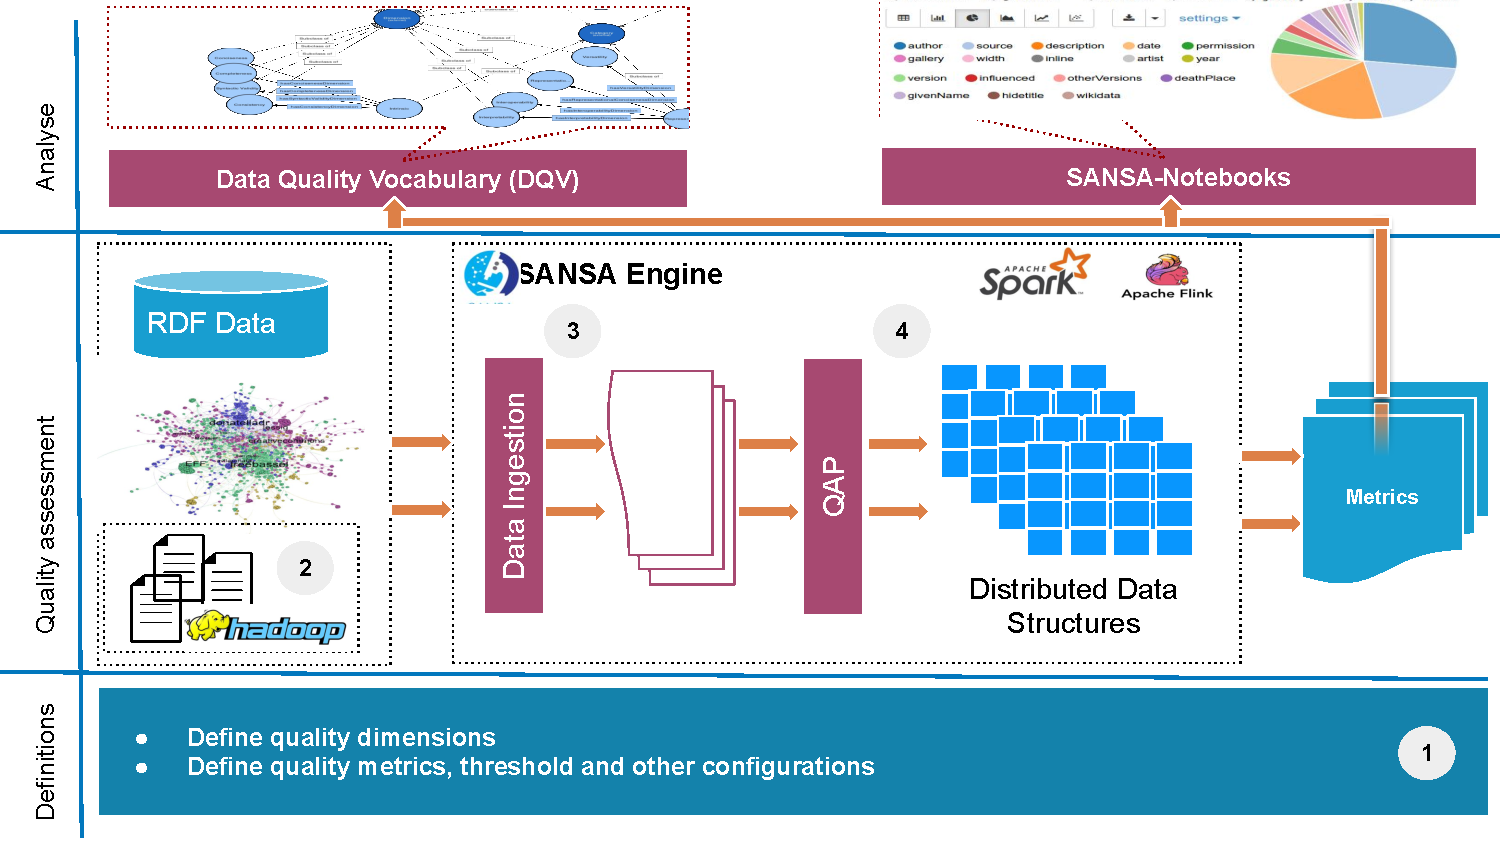
\includegraphics[width=1.0\columnwidth]{images/5_distqualityassessment/distqualityassessment-architecture.pdf}
\caption{\textbf{Overview of distributed quality assessment's abstract architecture}.
Main components of DistQualityAssessment: 1) Definitions -- defining quality metrics parameters, 2) Retrieving the RDF data, 3) Parsing and mapping RDF data into the main dataset (RDD of triples), and 4) Quality metric evaluation.}
\label{fig:DistQualityAssessmentSystem}
\end{figure*}
% source: https://docs.google.com/presentation/d/1JP_urfFpIzPKH4z1TXKSN3d00TmzbQ2YxGL7nQ7-IgI

\defn{Defining quality metrics parameters (Step 1)} The metric definitions are kept in a dedicated file that contains most of the configurations needed for the system to evaluate quality metrics and gather result sets.

\defn{Retrieving the \gls{RDF} data (Step 2)} \gls{RDF} data first needs to be loaded into a large-scale storage that Spark can efficiently read from.
We use \gls{HDFS}.
\gls{HDFS} is able to fit and stores any type of data in its Hadoop-native format and parallelizes them across a cluster while replicating them for fault tolerance.
In such a distributed environment, Spark automatically adopts different data locality strategies to perform computations as close to the needed data as possible in \gls{HDFS} and thus avoids data transfer overhead.
 
\defn{Parsing and mapping \gls{RDF} into the main dataset (Step 3)} We first create a distributed dataset called \emph{main dataset} that represent the \gls{HDFS} file as a collection of triples.
In Spark, this dataset is parsed and loaded into an \gls{RDD} of triples having the format 
\emph{Triple$<$(s,p,o)$>$}.

\defn{Quality metric evaluation (Step 4)} Considering the particular quality metric, Spark generates an execution plan, which is composed of one or more $\tau$ transformations and $\alpha$ actions. 
The numerical output of the final action is the quality of the input \gls{RDF} corresponding to the given metric.

\subsection{Implementation}
\label{subsection:distqualityassessment-implementation}
We have used the Scala\furl{https://www.scala-lang.org/} programming language \gls{API} in Apache Spark to provide the distributed implementation of the proposed approach. 

\begin{algorithm}
\caption{Spark-based parallel quality assessment algorithm.}
\label{alg:DistQualityAssessment}
\SetKwInOut{Input}{input}\SetKwInOut{Output}{output}
\Input{$RDF$: an RDF dataset,
	   $param$: quality metrics parameters.
      }
\Output{$dqv$ description or $metric$ numerical value}
    $\textit{triples} = spark.\textbf{rdf}(lang)(input)$ \label{line:qa-rdf2rdd} \\
    $\textit{triples}.persist()$ \label{line:qa-cache}\\
    $dqv \leftarrow \emptyset$ \\
    \ForEach{$m \in param.getListOfMetrics$}{
        $triples \leftarrow triples.Tranform~\{~t =>$ \label{line:qa-filter} \\
        $\quad \quad \textit{rule} \leftarrow m.Rule$ \\
        $\quad \quad t.apply(rule)~\}~$ \\
        $metric \leftarrow triples.apply(m.Action)$  \label{line:qa-action}\\
        \If{m.hasDQVdescription}{
            $dqvify \leftarrow metric.dqvify()$ \label{line:dqvify}
        }
        $dqv.add(dqvify)$
    }
\Return{$(dqv, metric)$} \label{line:qa-result}
\end{algorithm}

The DistQualityAssessment (see Algorithm~\ref{alg:DistQualityAssessment}) constructs the \emph{main dataset} (Line \ref{line:qa-rdf2rdd}) while reading \gls{RDF} data (e.g. NTriples file or any other \gls{RDF} serialization format) and converts it into an \gls{RDD} of triples.
This latter undergoes the transformation operation of applying the filtering through rules in $R$ and producing a new \emph{filtered} \gls{RDD} ($\mathcal{G'}$) (Line \ref{line:qa-filter}).
At the end, $\mathcal{G'}$ will serve as an input to the next step which applies a set of $\alpha$ actions (Line \ref{line:qa-action}).
The output of this step is the metric output represented as a numerical value (Line \ref{line:qa-action}). 
The result set of different quality metrics (Line \ref{line:qa-result}) can be further visualized and monitored using SANSA-Notebooks~\cite{iermilov-2017-sansa-iswc-demo}.\\
The user can also choose to extract the output in a machine-readable format (Line \ref{line:dqvify}). 
We have used the data quality vocabulary (DQV)~\cite{Isaac:16:dqv} to represent the quality metrics. 

Furthermore, we also provide a Docker image of the system integrated within the BDE platform\furl{https://github.com/big-data-europe} - an open-source Big Data processing platform allowing users to install numerous big data processing tools and frameworks and create working data flow applications.

The work done here (available under \textit{Apache License 2.0}) has been integrated into SANSA~\cite{lehmann-2017-sansa-iswc}, an open source\furl{https://github.com/SANSA-Stack} \emph{data flow processing engine} for scalable processing of large-scale \gls{RDF} datasets. 
SANSA uses Spark offering fault-tolerant, highly available and scalable approaches to process massive sized datasets efficiently. 
SANSA provides the facilities for semantic data representation, querying, inference, and analytics at scale.
Being part of this integration, DistQualityAssessment can take advantage of having the same user community as well as infrastructure build via the SANSA project.
Doing so, it can also ensure the sustainability of the tool given that SANSA is supported by several grants until at least 2021.

\paragraph{\textbf{Complexity Analysis}}
We deem that the overall time complexity of the distributed quality assessment evaluation is $O(n)$.
The performance of metrics computation depends on data shuffling (while filtering using rules in $R$) and data scanning. 
Our approach performs a direct mapping of any quality metric designed using $\mathcal{QAP}$ into a sequence of Spark-compliant Scala-commands, as a consequence, most of the operators used are a series of transformations like $map$, $filter$ and $reduce$.
The complexity of $map$ and $filter$ is considered to be linear with respect to the number of triples associated with it. 
The complexity of a metric then depends on the $\alpha$ operation that returns the count of the filtered output.
This later step works on the distributed \gls{RDD} between $p$ nodes which implies that the complexity of each node then becomes $O(n/p)$, where $n$ is a number of input triples.
Let be $O(\tau)$ a complexity of $\tau$, then the complexity of the metric will be $O(n/p*O(\tau))$.
This indicates that the runtime increases linearly when the size of an \gls{RDD} increases and decreases linearly when more nodes $p$ are added to the cluster.


\section{Evaluation}
\label{sec:distqualityassessment-evaluation}
The main aim of DistQualityAssessment is to serve massive large-scale real-life \gls{RDF} datasets. 
We are interested in addressing the following additional questions.

\begin{itemize}
    \item \textbf{Flexibility}: How fast our approach processes different types of metrics?
    \item \textbf{Scalability}: How large are the \gls{RDF} datasets that DistQualityAssessment can scale to? 
    What is the system speedup w.r.t the number of nodes in a cluster mode?
    \item \textbf{Efficiency}: How well our approach performs compared with other state-of-the-art systems on real-world datasets?
\end{itemize}
In the following, we present our experimental setup including the datasets used. 
Thereafter, we give an overview of our results.

\subsection{Experimental Setup}
We chose two real-world and one synthetic datasets for our experiments:
 \begin{enumerate}
 \item \emph{DBpedia}~\cite{dbpedia-swj} (v 3.9) -- a cross domain dataset.
 DBpedia is a knowledge base with a large ontology.
 We build a set of 3 pipelines of increasing complexity: (i) $M_{DBpedia}^{en}$ ($\approx$ 813M triples); (ii) $M_{DBpedia}^{de}$ ($\approx$ 337M triples); (iii) $M_{DBpedia}^{fr}$ ($\approx$ 341M triples). 
DBpedia has been chosen because of its popularity in the Semantic Web community.
\item \emph{LinkedGeoData}~\cite{SLHA11} -- a spatial \gls{RDF} knowledge base derived from OpenStreetMap.
\item \emph{Berlin \gls{SPARQL} Benchmark (BSBM})~\cite{Bizer2009TheBS}  -- a synthetic dataset based on an e-commerce use case containing a set of products that are offered by different vendors and reviews posted by consumers about products.
The benchmark provides a data generator, which can be used to create sets of connected triples of any particular size.
 \end{enumerate}
Properties of the considered datasets are given in Table~\ref{tab:qa-dataset_info}.

\begin{table*}
\centering
\begin{tabularx}{\textwidth}{Xcccccccc}	
\toprule
\multirow{2}{*}{$\longrightarrow$} & \multicolumn{1}{c}{} & \multicolumn{3}{c|}{DBpedia} & \multicolumn{4}{c}{BSBM} \\
\cline{3-9}  \rule{0pt}{10pt}
& LinkedGeoData & \scriptsize{en} & \scriptsize{de} & \scriptsize{fr}  & \scriptsize{2GB} &\scriptsize{20GB} &\scriptsize{200GB} &\\
\midrule
\scriptsize{\#nr. of triples}& \scriptsize{1,292,933,812} & \scriptsize{812,545,486} & \scriptsize{336,714,883} & \scriptsize{340,849,556} & \scriptsize{8,289,484} & \scriptsize{81,980,472} & \scriptsize{817,774,057} &  \\
\scriptsize{size (GB)} & \scriptsize{191.17} & \scriptsize{114.4} & \scriptsize{48.6} & \scriptsize{49.77} & \scriptsize{2} &\scriptsize{20} &\scriptsize{200} &\\
\bottomrule
\end{tabularx}
{\caption{\textbf{Dataset summary information (nt format)}.
Lists dataset information used on the evaluation of the DistQualityAssessment.
The size (in GB) and the number of triples are given.}
\label{tab:qa-dataset_info}}
\end{table*}

We implemented DistQualityAssessment using Spark-2.4.0, Scala 2.11.11 and Java 8, and all the data were stored on the \gls{HDFS} cluster using Hadoop 2.8.0.
The experiments in local mode are all performed on a single instance of the cluster.
Specifically, we compare our approach with Luzzu~\cite{debattista2016luzzu} v4.0.0, a state-of-the-art quality assessment system\furl{https://github.com/Luzzu/Framework}.
All distributed experiments were carried out on a small cluster of 7 nodes (1 master, 6 workers): Intel(R) Xeon(R) CPU E5-2620 v4 @ 2.10GHz (32 Cores), 128 GB RAM, 12 TB SATA RAID-5.
The machines were connected via a Gigabit network.
All experiments have been executed three times and the average value is reported in the results.

\subsection{Results}
%source: https://docs.google.com/spreadsheets/d/1RrwtYbJFhd2g8U4V5OTrWT1sd6ujtZopvWyAIIlJqnQ
We evaluate the proposed approach using the above datasets to compare it against Luzzu~\cite{debattista2016luzzu}.
We carry out two sets of experiments.
First, we evaluate the runtime of our distributed approach in contrast to Luzzu.
Second, we evaluate the horizontal scalability via increasing nodes in the cluster.
Results of the experiments are presented in Table~\ref{tbl:distqualityassessment-performance-evaluation}, Figure~\ref{fig:distqualityassessment-sizeup-scalability} and
\ref{fig:distqualityassessment-node-scalability}.
Based on the metric definition, some metrics make use of external access (e.g. Dereferenceability of Forward Links) which leads to a significant increase in Spark processing due to network latency. 
For the sake of the evaluation, we have suspended such metrics.
As of that, we choose seven metrics (see Table~\ref{tab:MetricRules} for more details) where the level of difficulty varies from simple to complex according to the combination of transformation/action operations involved.

\subsubsection{Performance evaluation on large-scale RDF datasets}
\label{subsubsection:distqualityassessment-large_scale_datasets}
We started our experiments by evaluating the \textit{speedup} gained by adopting a distributed implementation of quality assessment metrics using our approach, and compare it against Luzzu.
We run the experiments on five datasets
($DBpedia_{en}$, $DBpedia_{de}$, $DBpedia_{fr}$, $LinkedGeoData$ and $BSBM_{200GB}$).
Local mode represents a single instance of the cluster without any tuning of Spark configuration and the cluster mode includes further tuning.
Luzzu was run in a local environment on a single machine with two strategies: (1) streaming the data for each metric separately, and (2) one stream/load -- all metrics evaluated just once. 

\begin{table*}
\centering
\begin{tabularx}{\textwidth}{Xcccccc}	
\toprule
\multicolumn{1}{l}{}& \multicolumn{5}{c}{\scriptsize{Runtime (m)} (\scriptsize{mean/std})} \\
\cline{2-6}
\rule{0pt}{8pt}
\multirow{2}{*}{$\longrightarrow$} & \multicolumn{2}{c|}{\scriptsize{\textbf{Luzzu}}} & \multicolumn{3}{c}{\scriptsize{\textbf{DistQualityAssessment}}} \\
\cline{2-6}  \rule{0pt}{10pt}
& \scriptsize{a) single} & \scriptsize{b) joint}  & \scriptsize{c) local} & \scriptsize{d) cluster} & \scriptsize{e) speedup ratio w.r.t} \\
& & & & & \scriptsize{Luzzu \textbar DistQualityAssessment$^{c)}$} \\
\midrule
\multirow{5}{*}{\rotatebox{90}{\textbf{Large-scale}}}
$LinkedGeoData$ & \textcolor{red}{\scriptsize{Fail}} & \textcolor{red}{\scriptsize{Fail}} & \scriptsize{446.9/63.34} & \win \scriptsize{7.79/0.54} & \win \scriptsize{n/a\textbar56.4x}\\
\hspace{0.2cm} $DBpedia_{en}$ & \textcolor{red}{\scriptsize{Fail}} & \textcolor{red}{\scriptsize{Fail}} & \scriptsize{274.31/38.17} & \win \scriptsize{1.99/0.04} & \win \scriptsize{n/a\textbar136.8x} \\
\hspace{0.2cm} $DBpedia_{de}$ & \textcolor{red}{\scriptsize{Fail}} & \textcolor{red}{\scriptsize{Fail}} & \scriptsize{161.4/24.18} & \win \scriptsize{0.46/0.04} & \win \scriptsize{n/a\textbar349.9x}\\
\hspace{0.2cm} $DBpedia_{fr}$ & \textcolor{red}{\scriptsize{Fail}} & \textcolor{red}{\scriptsize{Fail}} & \scriptsize{195.3/26.16} & \win \scriptsize{0.38/0.04} & \win \scriptsize{n/a\textbar512.9x}\\
\hspace{0.2cm} $BSBM_{200GB}$ & \textcolor{red}{\scriptsize{Fail}} & \textcolor{red}{\scriptsize{Fail}} & \scriptsize{454.46/78.04} & \win \scriptsize{7.27/0.64} & \win \scriptsize{n/a\textbar61.5x}\\
\midrule
\multirow{10}{*}{\rotatebox{90}{\textbf{Small to medium}}}
$BSBM_{0.01GB}$ & \scriptsize{2.64/0.02} & \scriptsize{2.65/0.01} & \win \scriptsize{0.04/0.0} & \scriptsize{0.42/0.04} & \win \scriptsize{65x\textbar (-0.9x)}\\
\hspace{0.2cm} $BSBM_{0.02GB}$ & \scriptsize{5.9/0.16} & \scriptsize{5.66/0.02} & \win \scriptsize{0.04/0.0} & \scriptsize{0.43/0.03} & \win \scriptsize{146.5x\textbar (-0.9x)}\\
\hspace{0.2cm} $BSBM_{0.05GB}$ & \scriptsize{16.38/0.44} & \scriptsize{15.39/0.21} & \win \scriptsize{0.05/0.0} & \scriptsize{0.46/0.02} & \win \scriptsize{326.6x\textbar (-0.9x)}\\
\hspace{0.2cm} $BSBM_{0.1GB}$ & \scriptsize{40.59/0.56} & \scriptsize{37.94/0.28} & \win \scriptsize{0.06/0.0} & \scriptsize{0.44/0.05} & \win \scriptsize{675.5x\textbar (-0.9x)}\\
\hspace{0.2cm} $BSBM_{0.2GB}$ & \scriptsize{101.8/0.72} & \scriptsize{101.78/0.64} & \win \scriptsize{0.07/0.0} & \scriptsize{0.4/0.03} & \win \scriptsize{1453.3\textbar (-0.8x)}\\
\hspace{0.2cm} $BSBM_{0.5GB}$ & \scriptsize{459.19/18.72} & \scriptsize{468.64/21.7} & \win \scriptsize{0.15/0.01} & \scriptsize{0.48/0.03} & \win \scriptsize{3060.3x\textbar (-0.7x)}\\
\hspace{0.2cm} $BSBM_{1GB}$ & \scriptsize{1454.16/10.55} & \scriptsize{1532.95/51.6} & \win \scriptsize{0.4/0.02} & \scriptsize{0.56/0.02} & \win \scriptsize{3634.4x\textbar (-0.3x)}\\
\hspace{0.2cm} $BSBM_{2GB}$ & \textcolor{blue}{\scriptsize{Timeout}} & \textcolor{blue}{\scriptsize{Timeout}} & \scriptsize{3.19/0.16} & \win \scriptsize{0.62/0.04} & \win \scriptsize{n/a\textbar 4.1x}\\
\hspace{0.2cm} $BSBM_{10GB}$ & \textcolor{blue}{\scriptsize{Timeout}} & \textcolor{blue}{\scriptsize{Timeout}} & \scriptsize{29.44/0.14} & \win \scriptsize{0.52/0.01} & \win \scriptsize{n/a\textbar 55.6x}\\
\hspace{0.2cm} $BSBM_{20GB}$ & \textcolor{red}{\scriptsize{Fail}} & \textcolor{red}{\scriptsize{Fail}} & \scriptsize{34.32/9.22} & \win \scriptsize{0.75/0.29} & \win \scriptsize{n/a\textbar 44.8x}\\
\bottomrule
\end{tabularx}
{\caption{\textbf{Performance evaluation on large-scale RDF datasets}.
A \textit{speedup} analysis gained by DistQualityAssessment as compared with Luzzu.
The experiments were run on five datasets
($DBpedia_{en}$, $DBpedia_{de}$, $DBpedia_{fr}$, $LinkedGeoData$ and $BSBM_{200GB}$).
Luzzu was run in a local environment on a single machine with two strategies: (1) streaming the data for each metric separately, and (2) one stream/load -- all metrics evaluated just once.
}
\label{tbl:distqualityassessment-performance-evaluation}}
\end{table*}

Table~\ref{tbl:distqualityassessment-performance-evaluation} shows the performance of two approaches applied to five datasets.
In Table~\ref{tbl:distqualityassessment-performance-evaluation} we indicate "Timeout" whenever the process did not complete within a certain amount of time\f{We set the timeout delay to 24 hours of the quality assessment evaluation stage.} and "Fail" when the system crashed before this timeout delay.
%Fail message : Exception in thread "main" org.apache.jena.ext.com.google.common.util.concurrent.ExecutionError: java.lang.OutOfMemoryError: GC overhead limit exceeded
Column Luzzu$^{a)}$ represents the performance of Luzzu on bulk load -- considering each metric as a sequence of the execution, on the other hand, the column Luzzu$^{b)}$ reports on the performance of Luzzu using a joint load by evaluating each metric using one load.
The last columns reports on the performance of DistQualityAssessment run on a local mode $c)$, cluster mode $d)$ and speedup ratio of our approach compared to Luzzu$^{b)}$ ($d)/b)-1$) and itself evaluated on local mode ($d)/c)-1$) is reported on the column $e)$.
We observe that the execution of our approach finishes with all the datasets whereas this is not the case with Luzzu which either timeout or fail at some point.

Unfortunately, Luzzu was not capable of evaluating the metrics over large-scale \gls{RDF} datasets from Table~\ref{tbl:distqualityassessment-performance-evaluation} (part one). 
For that reason, we run yet another set of experiments on very small datasets that Luzzu was able to handle. 
The second part of the Table~\ref{tbl:distqualityassessment-performance-evaluation} shows a performance evaluation of our approach compared with Luzzu on very small \gls{RDF} datasets.
In some cases (e.g. \ref{qm:RC1}, \ref{qm:SV3}) for a very small dataset, Luzzu performs better than our approach with a small margin of runtime in the local mode.
It is due to the fact that in the streaming model when Luzzu$^{a)}$ finds the first statement which fulfills the condition (e.g.finding the shortest \gls{URI}s), it stops the evaluation and returns the results.
On the contrary, our approach evaluates the metrics over the whole dataset exploiting the fault-tolerance and resilient features build-in Spark.
In other cases, Luzzu suffers from significant slowdowns, which are several orders of magnitude slower.
Therefore, its average runtime over all metrics is worst as compared to our approach. 
It is important to note that our approach to these very small datasets degrades while running on the cluster mode.
This is because of the network overhead while shuffling the data, but it outperforms Luzzu$^{a),b)}$ when considering ''average runtime'' over all the metrics (even for very small datasets).

Findings shown in Table~\ref{tbl:distqualityassessment-performance-evaluation} depicts that our approach starts outperforming when the size of the dataset grows (e.g. $BSBM_{2GB}$).
The runtime in the cluster mode stays constant when the size of the data fits into the main memory of the cluster.
On other hand, Luzzu is not able to evaluate the metrics when the size of data starts increasing, the time taken lasts beyond the delay we set for small datasets. 
Because of the large differences, we have used a logarithmic scale to better visualize these results.

\subsubsection{Scalability performance analysis}
\label{subsubsection:distqualityassessment-scalability_performance}
In this experiment, we evaluate the efficiency of our approach.
Figure~\ref{fig:distqualityassessment-sizeup-scalability} and \ref{fig:distqualityassessment-node-scalability} illustrates the results of the comparative efficiency analysis.

\begin{figure*}
\centering
 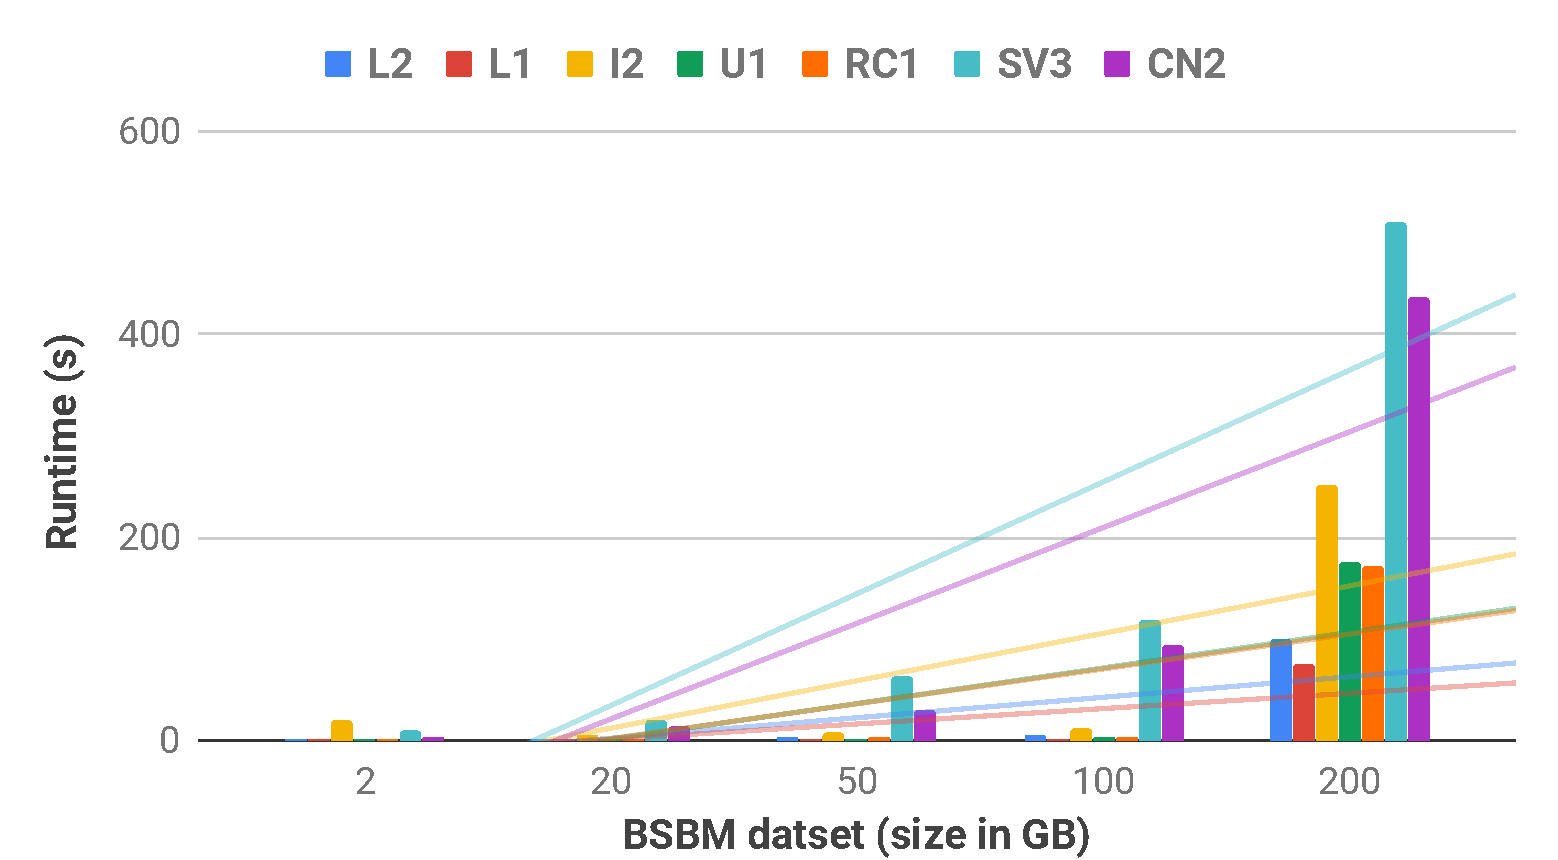
\includegraphics[width=1.0\columnwidth]{images/5_distqualityassessment/distqualityassessment-sizeup-scalability.pdf}
    \caption{\textbf{Sizeup performance evaluation of DistQualityAssessment}.
    The analysis fixes the number of nodes to 6 and grows the size of datasets to measure whether DistQualityAssessment can deal with larger datasets.
    We see that the execution time increases linearly and is near-constant when the size of the dataset increases. 
    As expected, it stays near-constant as long as the data fits in memory.}
    \label{fig:distqualityassessment-sizeup-scalability}
\end{figure*}

\textit{Data scalability} 
To measure the performance of \textit{size-up} scalability of our approach, we run experiments on five different sizes.

We fix the number of nodes to 6 and grow the size of datasets to measure whether DistQualityAssessment can deal with larger datasets.
For this set of experiments, we consider BSBM benchmark tool to generate synthetic datasets of different sizes since the real-world dataset is considered to be unique in their size and attributes.

We start by generating a dataset of 2GB.
Then, we iteratively increase the size of datasets.
On each dataset, we run our approach and the runtime is reported on Figure~\ref{fig:distqualityassessment-sizeup-scalability}.
The $x$-axis shows the size of the BSBM dataset with an increasing order of 10x magnitude.

By comparing the runtime (see Figure~\ref{fig:distqualityassessment-sizeup-scalability}), we note that the execution time increases linearly and is near-constant when the size of the dataset increases.
As expected, it stays near-constant as long as the data fits in memory.
This demonstrates one of the advantages of utilizing the in-memory approach for performing quality assessment computation.
The overall time spent in data read/write and network communication found in disk-based approaches is saved.
However, when the data overflows the memory, and it is spilled to disk, the performance degrades.
These results show the scalability of our algorithm in the context of size-up.

\textit{Node scalability} In order to measure node scalability, we vary the number of workers on our cluster.
The number of workers has varied from 1, 2, 3, 4 and 5 to 6.

\begin{figure*}
\centering
  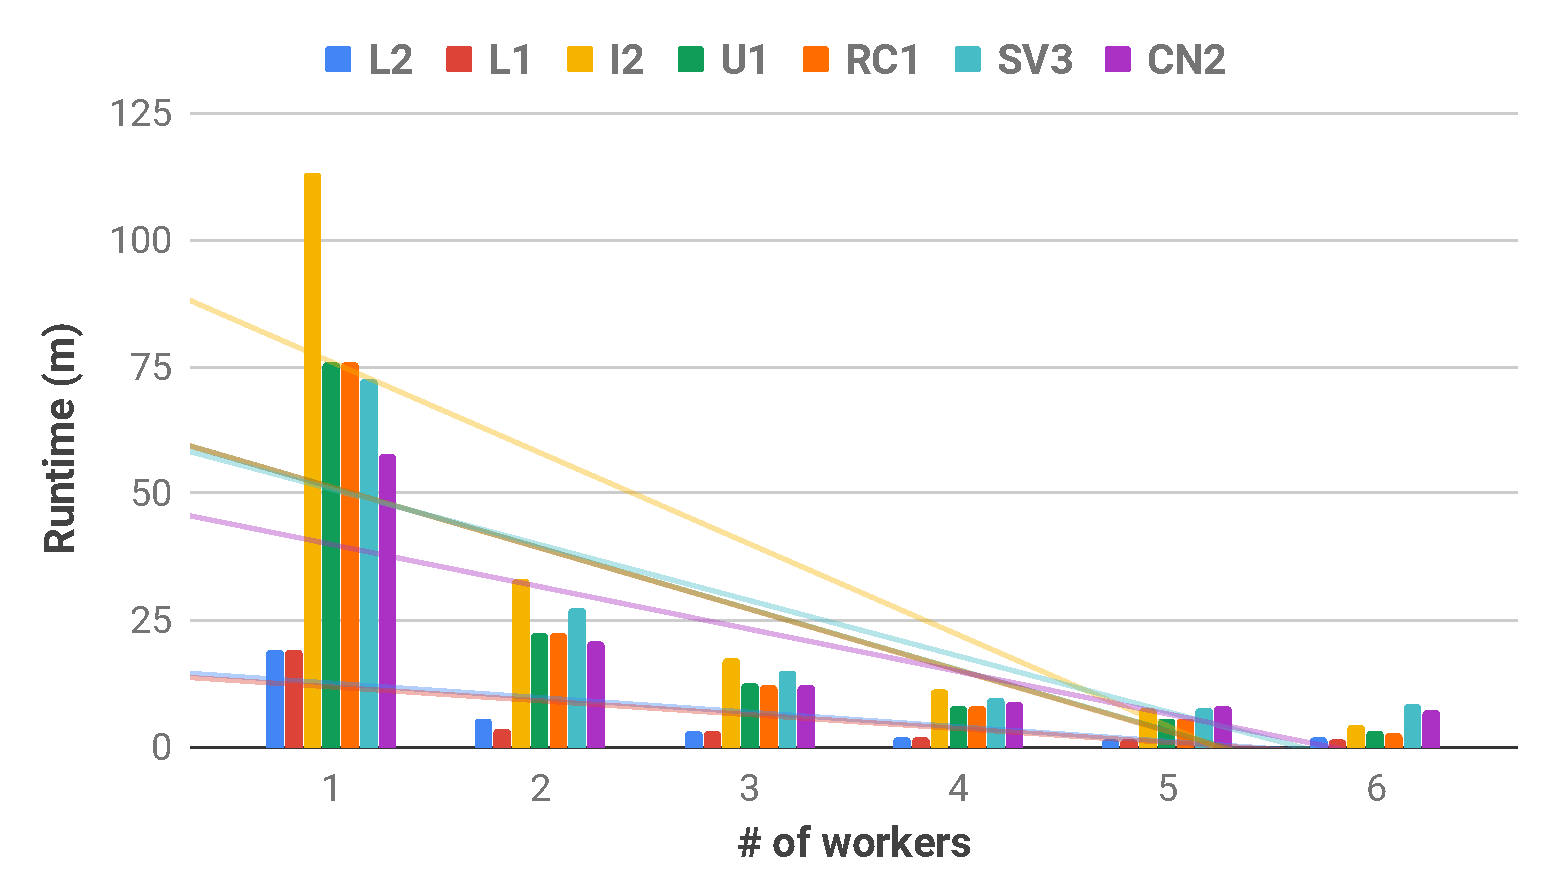
\includegraphics[width=1.0\columnwidth]{images/5_distqualityassessment/distqualityassessment-node-scalability.pdf}
    \caption{\textbf{Node scalability performance evaluation of DistQualityAssessment}.
    The analysis keeps the size of the dataset constant ($BSBM_{200GB}$) and varies the number of workers on the cluster.
    The number of workers varies from 1, 2, 3, 4 and 5 to 6.
    We can see that as the number of workers increases, the execution time cost-decrease is almost linear. 
    It decreases about 14 times (from 433.31 minutes down to 28.8 minutes) as cluster nodes increase from one to six worker nodes. The results shown here imply that our approach can achieve near-linear scalability in performance in the context of speedup.}
    \label{fig:distqualityassessment-node-scalability}
\end{figure*}

Figure~\ref{fig:distqualityassessment-node-scalability} shows the speedup for $BSBM_{200GB}$ with the various number of worker nodes.
We can see that as the number of workers increases, the execution time cost-decrease is almost linear.
The execution time decreases about 14 times (from 433.31 minutes down to 28.8 minutes) as cluster nodes increase from one to six worker nodes.
The results shown here imply that our approach can achieve near-linear scalability in performance in the context of speedup.

Furthermore, we conduct the effectiveness evaluation of our approach.
Speedup $S$ is an important metric to evaluate a parallel algorithm.
It is defined as a ratio $S=T_s/T_n$, where $T_s$ represents the execution time of the algorithm run on a single node and $T_n$ represents the execution time required for the same algorithm on $n$ nodes with the same configuration and resources.
Efficiency is defined as a ratio $E = S/n =T_s/n T_n$ which measures the processing power being used, in our case the speedup per node.

\begin{figure*}
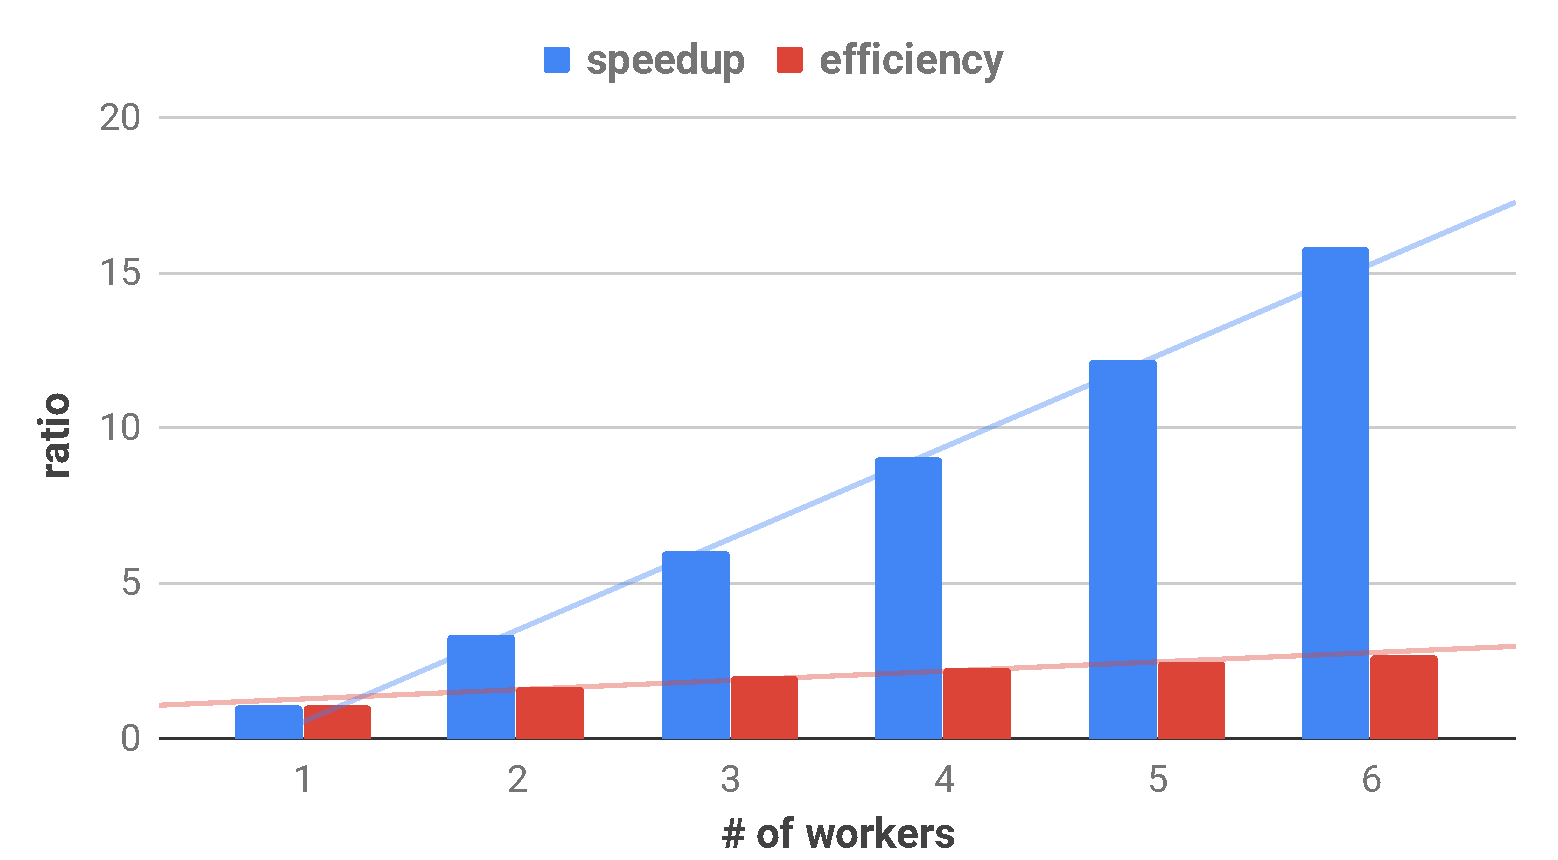
\includegraphics[width=1.0\columnwidth]{images/5_distqualityassessment/distqualityassessment-effectiveness.pdf}
\caption{\textbf{Effectiveness of DistQualityAssessment}.
The speedup performance trend shows that it achieves almost linear speedup and even superlinear in some cases.
The speedup grows faster than the number of worker nodes due to the computation task for the metric being computationally intensive, and the data does not fit in the cache when executed on a single node but fits into several machines when the workload is divided amongst the cluster for parallel evaluation.
}
\label{fig:distqualityassessment-effectiveness}
\end{figure*}

The speedup and efficiency curves of DistQualityAssessment are shown in Figure~\ref{fig:distqualityassessment-effectiveness}.
The trend shows that it achieves almost linear speedup and even superlinear in some cases.
The upper curve in the Figure~\ref{fig:distqualityassessment-effectiveness} indicates superlinear speedup. 
The speedup grows faster than the number of worker nodes.
This is due to the computation task for the metric being computationally intensive, and the data does not fit in the cache when executed on a single node. 
But it fits into the caches of several machines when the workload is divided amongst the cluster for parallel evaluation.
While using Spark, the superlinear speedup is an outcome of the improved complexity and runtime, in addition to efficient memory management behavior of the parallel execution environment.

\subsubsection{Correctness of metrics}
In order to test the correctness of implemented metrics, we assess the numerical values for metrics like \ref{qm:L1}, \ref{qm:L2}, and \ref{qm:RC1} on very small datasets and the results are found correct w.r.t Luzzu. 
For metrics like \ref{qm:I2} and \ref{qm:CN2}, Luzzu uses approximate values for faster performance, and that is not the same as getting the exact number as in the case of our implementation.

\subsubsection{Overall analysis by metrics}
We analyze the overall run-time of the metric evaluation.
Figure~\ref{fig:distqualityassessment-overall-analysis} reports on the run-time of each metric considered (see Table~\ref{tab:MetricRules}) on both $BSBM_{20GB}$ and $BSBM_{200GB}$ datasets.

\begin{figure*}
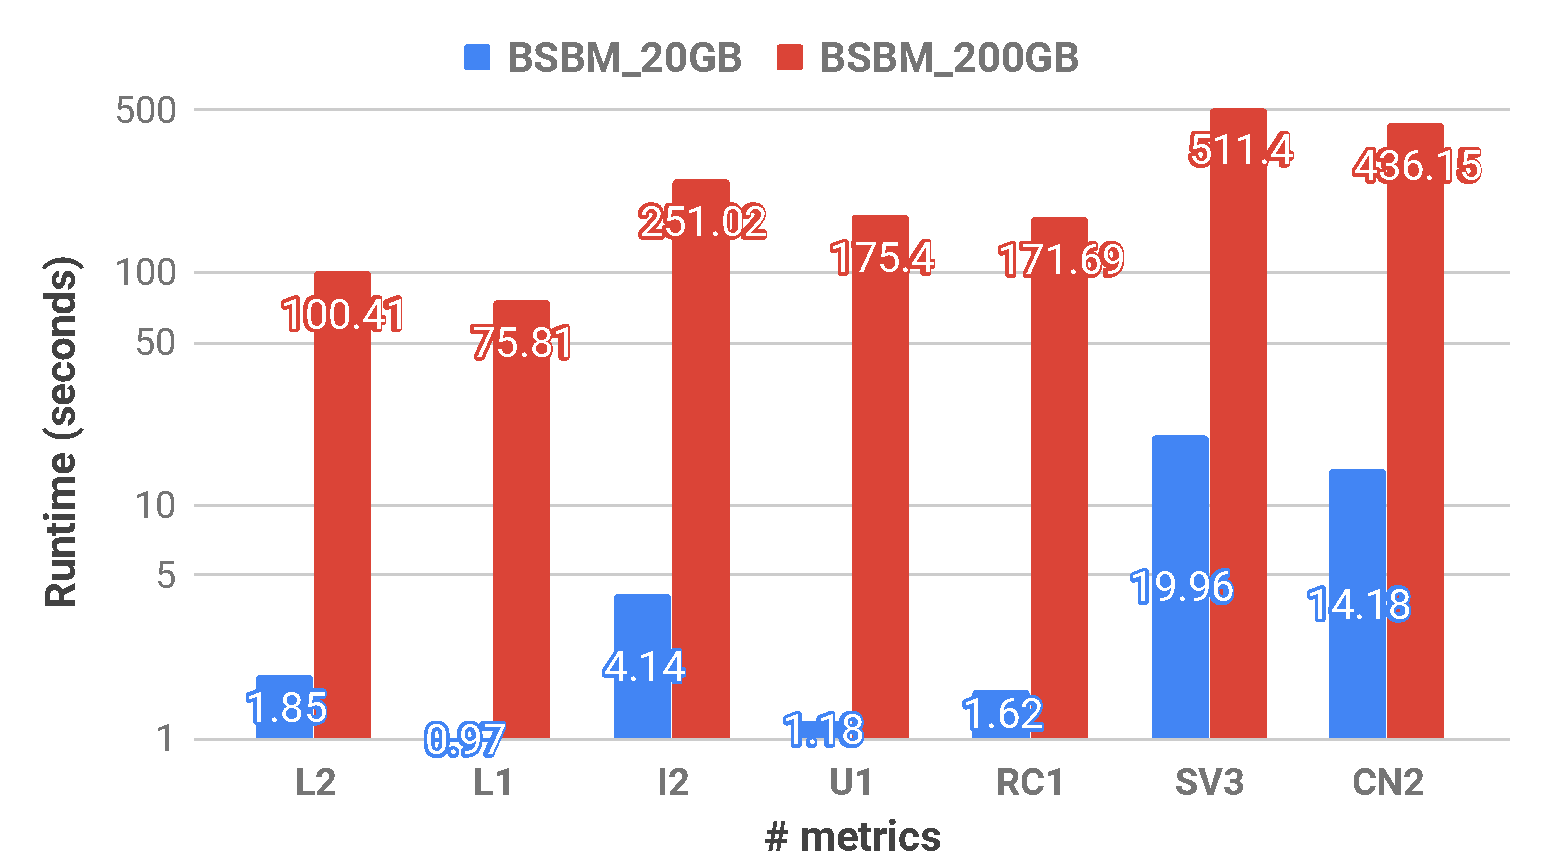
\includegraphics[width=1.0\columnwidth]{images/5_distqualityassessment/distqualityassessment-overall-analysis.pdf}
\caption{\textbf{Overall analysis of by metric in the cluster mode (log scale)}.
It shows that the execution is sometimes a little longer when there is a shuffling involved in the cluster compared to when data is processed without movement e.g. Metric L2 and L1. 
Metric SV3 and CN2 are the most expensive ones in terms of runtime. This is due to the extra overhead caused by extracting the literals for objects and checking the lexical form of its datatype.
}
\label{fig:distqualityassessment-overall-analysis}
\end{figure*}

DistQualityAssessment implements predefined quality assessment metrics from \cite{zaveri2015quality}. 
We have implemented these metrics in a distributed manner such that most of them have a run-time complexity of $O(n)$ where $n$ is the number of input triples.
The overall performance of analysis for the BSBM dataset with two instances is shown in Figure~\ref{fig:distqualityassessment-overall-analysis}.
The results obtained show that the execution is sometimes a little longer when there is a shuffling involved in the cluster compared to when data is processed without movement e.g.~Metric \ref{qm:L2} and \ref{qm:L1}.
Metric~\ref{qm:SV3} and \ref{qm:CN2} are the most expensive ones in terms of runtime.
This is due to the extra overhead caused by extracting the literals for objects, and checking the lexical form of its datatype. 

Overall, the evaluation study carried out demonstrates that distributed computation of  different quality measures is scalable and the execution ends in reasonable time given the large volume of data.


\section{Summary}
\label{sec:distqualityassesment-summary}
The data quality assessment becomes challenging with the increasing sizes of data.
Many existing tools mostly contain a customized data quality functionality to detect and analyze data quality issues within their own domain. 
However, this process is both data-intensive and computing-intensive and it is a challenge to develop fast and efficient algorithms that can handle large scale \gls{RDF} datasets.

In this thesis, we have introduced DistQualityAssessment, a novel approach for distributed in-memory evaluation of \gls{RDF} quality assessment metrics implemented on top of the Spark framework.
The presented approach offers generic features to solve common data quality checks.
As a consequence, this can enable further applications to build trusted data utilities. 

We have demonstrated empirically that our approach improves upon the previous centralized approach that we have compared against.
The benefit of using Spark is that its core concepts (\gls{RDD}s) are designed to scale horizontally. 
Users can adapt the cluster sizes corresponding to the data sizes, by dropping when it is not needed and adding more when there is a need for it.